\chapter{Implementation of OpenAPI Fuzzer}
In this chapter we discuss the implementation details and internals of our fuzzer. We will take a look at the different libraries that helped us along the way as well as some interesting features of the programming language we used.

OpenAPI fuzzer is implemented in Rust programming language. Rust is a strongly and statically typed systems programming language. Which is in contrast with the dynamic programming language all before mentioned fuzzers are implemented in - Python. Moreover, Rust possesses features from functional programming language that helped us during the implementation.

\paragraph{}
Right after the OpenAPI Fuzzer starts it, parses the command line arguments (full help information can be seen in figure \ref{fig:openapi-fuzzer-help}) and proceeds to parsing the OpenAPI specification. The OpenAPI Fuzzer represents the specification by structs rather than some more dynamic datastructure like hashmap which was the case of TnT-Fuzz. Thanks to this decision and use of algebrainc datatypes it was way easier for us to handle all the corner cases of OpenAPI specification. For example when some field was not present in a specification where TnT-Fuzz expected it, it raised and exception and failed to run. For the maping between specification and Rust's structs we utilized a \texttt{openapiv3} Rust library \cite{openapiv32020github}.

\begin{figure}
\begin{verbatim}
Usage: openapi-fuzzer -s <spec> -u <url> [-i <ignore-status-code>] [-H <header>]

OpenAPI fuzzer

Options:
    -s, --spec                 path to OpenAPI specification
    -u, --url                  url of api to fuzz
    -i, --ignore-status-code   status codes that will not be considered as finding
    -H, --header               additional header to send
    --help                     display usage information
\end{verbatim}
\caption{OpenAPI Fuzzer help message}
\label{fig:openapi-fuzzer-help}
\end{figure}

Another issue we came across was resolving \textit{components} section of the specification that we described in section \ref{subsec:components}. We needed to assign an object located in \textit{components} section to every reference located eslewhere in the specification. We dealth with this issue by using \texttt{openapi\_utils} \cite{openapiutils2020github} library which possesses this functionality. Moreover, the dereferencing is done only once before the startup of the program, so it will not start until correct specification is provided. We also contributed to this project a feature that enables it to accept more valid specification and thus produces less true negative results.

For a random payload  generation we are using a library called \texttt{arbitrary} \cite{arbitrary2020github} which is able to create a structured data (like strings, floats or integers) from instructured input - random bytes. Arbitrary makes the input creation look trivial. Futhermore, due clever use of generic programming in a \texttt{rand} library \cite{rand2020github} we generate strings that may contain any unicode character, rather that an ascii ones, which was the case of previously described fuzzzers.

Before sending requests user is able to supply an additional header or overwrite an existing one by specifying it by command line option. Additionally, we decided to use operating system's certificates instead of the ones that are used by deafault by our chosen library for sending HTTP requests. The use of native certificates enabled us to crate HTTPS connections which was required by some applications we tested like Kubernetes.

The next step after sending and determining wheter a request triggered a bug is an error reporting. When the OpenAPI Fuzzer fings a bug it stores the request in a JSON format. We chose the JSON format since it is considered to be a de facto standard when serializing data and thererore it is easier for other programs to further process it. Moreover, the fuzzer creates a directory structure that corresponds to the OpenAPI specification. An example of such a structure is shown in a figure \ref{fig:openapi-fuzzer-results} (created ty \texttt{tree} command). The root directory is called \texttt{results} and contains subdirectories corresponding to the endpoints of the API. Then they are followed by HTTP methods used when quering the resource and HTTP status codes received from the resource. Lastly, the directories named after received HTTP status code contains JSON files with saved requests. Due to this structure user is able to focuss only on certain type of bug when reproducing and debugging an API.

\begin{figure}[h]
\begin{verbatim}
results/
|-- notifications
|   \-- GET
|       \-- 422
|-- user-applications-oauth2-{id}
|   |-- DELETE
|   |   \-- 500
|   \-- PATCH
|       \-- 500
\-- user-times
    \-- GET
        \-- 422
\end{verbatim}
\caption{Directory structure of findings produced by OpenAPI Fuzzer}
\label{fig:openapi-fuzzer-results}
\end{figure}

Finally, to make the fuzzing experience more pleasant and informative for the user, OpenAPI fuzzer displays the progress in a TUI. The OpenAPI Fuzzer's TUI can be seen in a figure \ref{fig:openapi-fuzzer-run}. It displays the progress in several columns. The first one corresponds to the fuzzed endpoint and others represent the HTTP methods used to query the endpoint. The cells include two counters. The number of successful request out of total number of requests sent to an endpoint with corresponding HTTP method. Further, the number of successful requests is denoted by red collor to be easier to notice. Additionally, it may happen that an API has so many endpoint that they will not fit on the screen. For that reason we implemented a scolling in the TUI. User can use arrow keys to move by up and down by a line or use some handy keyboard shortcuts like \textit{Home} and \textit{End} to move to the first and last endpoint.

For the implementation of the TUI we used a \texttt{tui-rs} \cite{tuirs2020github} with similar functionality to well-known \texttt{ncurses} library. However, the \texttt{tui-rs}, unlike \texttt{ncurses} offers different rendering basckends. The backed of our choice is called a \texttt{crossterm} \cite{crossterm2020github}. The use of the \texttt{crossterm} backend enables the OpenAPI Fuzzer to run across all mainstream operating systems without a difference.

\begin{figure}
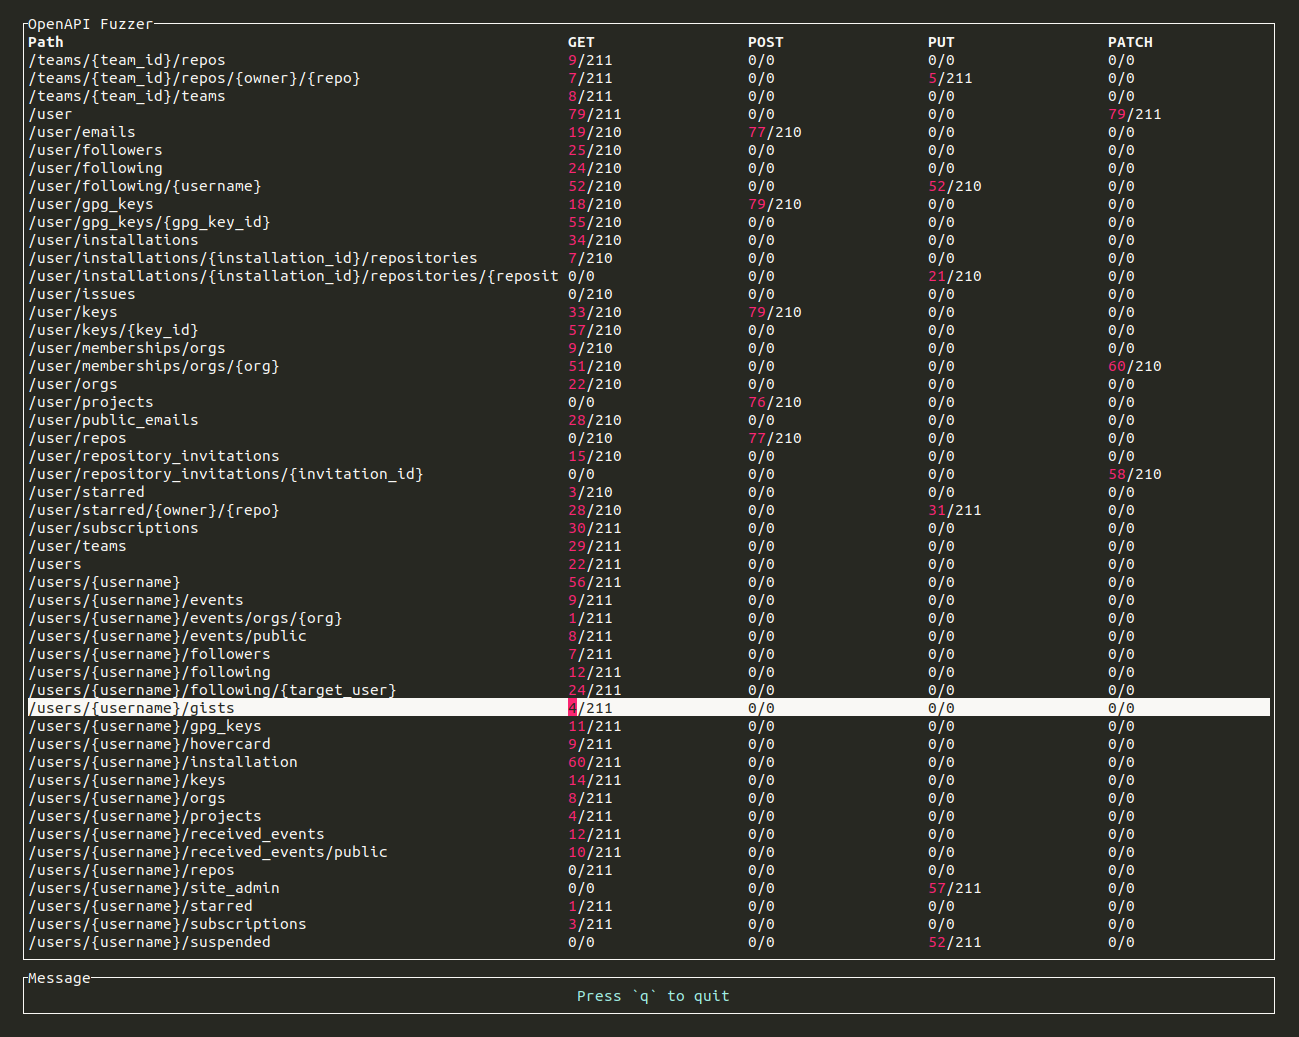
\includegraphics[width=\textwidth]{demo}
\caption{OpenAPI Fuzzer running}
\label{fig:openapi-fuzzer-run}
\end{figure}

\paragraph{}
Now that we know the internal structure and architecture of the OpenAPI Fuzzer, it is time to test it. In the next chapter we will present results we achieved when we were fuzzing some well known and battle-tested APIs.
